\begin{figure}[t]
\centering
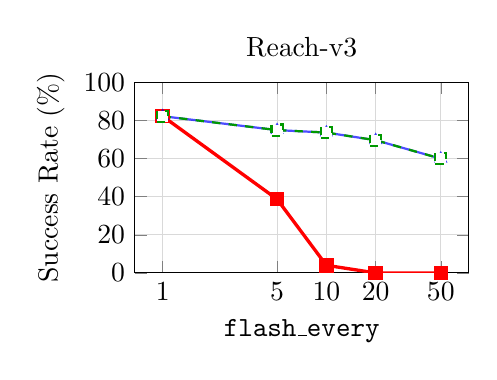
\begin{tikzpicture}
\begin{axis}[
    name=plot1,
    width=0.48\textwidth,
    height=4cm,
    xlabel={\texttt{flash\_every}},
    ylabel={Success Rate (\%)},
    title={\task{Reach-v3}},
    xmode=log,
    log basis x=10,
    xtick={1,5,10,20,50},
    xticklabels={1,5,10,20,50},
    ymin=0, ymax=100,
    grid=major,
    grid style={gray!30},
]
\addplot[red, mark=square*, very thick] coordinates {(1,82.3) (5,38.7) (10,4.0) (20,0.0) (50,0.0)};
\addplot[blue, mark=triangle*, thick, opacity=0.7] coordinates {(1,82.3) (5,75.0) (10,73.7) (20,69.7) (50,60.0)};
\addplot[green!60!black, mark=square*, mark options={fill=white}, thick, dashed] coordinates {(1,82.3) (5,75.0) (10,73.7) (20,69.7) (50,60.0)};
\end{axis}
\end{tikzpicture}
\hfill
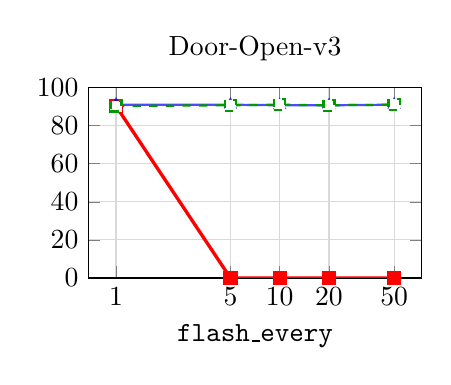
\begin{tikzpicture}
\begin{axis}[
    width=0.48\textwidth,
    height=4cm,
    xlabel={\texttt{flash\_every}},
    title={\task{Door-Open-v3}},
    xmode=log,
    log basis x=10,
    xtick={1,5,10,20,50},
    xticklabels={1,5,10,20,50},
    ymin=0, ymax=100,
    grid=major,
    grid style={gray!30},
]
\addplot[red, mark=square*, very thick] coordinates {(1,90.3) (5,0.0) (10,0.0) (20,0.0) (50,0.0)};
\addplot[blue, mark=triangle*, thick, opacity=0.7] coordinates {(1,91.0) (5,91.0) (10,90.7) (20,90.7) (50,91.0)};
\addplot[green!60!black, mark=square*, mark options={fill=white}, thick, dashed] coordinates {(1,90.3) (5,90.7) (10,91.0) (20,90.7) (50,91.0)};
\end{axis}
\end{tikzpicture}
\par\vspace{1mm}
\begin{tikzpicture}[baseline]
\draw[red, very thick] (0,0) -- (0.45,0);
\node[draw=red, fill=red, rectangle, inner sep=1.6pt] at (0.225,0) {};
\node[anchor=west, font=\scriptsize] at (0.55,0) {NoMemory};

\draw[blue, thick, opacity=0.7] (2.2,0) -- (2.65,0);
\node[draw=blue, fill=blue, regular polygon, regular polygon sides=3, inner sep=1.8pt] at (2.425,0) {};
\node[anchor=west, font=\scriptsize] at (2.75,0) {TextBuffer};

\draw[green!60!black, thick, dashed] (5.1,0) -- (5.55,0);
\node[draw=green!60!black, fill=white, rectangle, inner sep=1.6pt] at (5.325,0) {};
\node[anchor=west, font=\scriptsize] at (5.65,0) {StructMemory};
\end{tikzpicture}
\caption{Memory requirement curves on Reach-v3 and Door-Open-v3. The x-axis shows sampled \texttt{flash\_every} values $\{1,5,10,20,50\}$ on a log scale. NoMemory degrades as goal flashes become rarer, while TextBuffer and StructMemory remain near FO. On Door-Open-v3, NoMemory collapses already at \texttt{flash\_every}$=$5, and TextBuffer/StructMemory overlap throughout.}
\label{fig:flash_every}
\end{figure}
